\documentclass[11pt]{article} 

\usepackage[utf8]{inputenc} 

\usepackage{graphicx}

\usepackage{geometry}

\setlength{\parindent}{0cm}

\geometry{a4paper} 


\title{Winterthur Yard: Abschlussbericht Projekt}
\author{Maja Fritschi, Raphael Spörri, Florian Bosshard}
\date{} 

\begin{document}

\maketitle

\tableofcontents
\newpage

\section{Applikation}
Die aktuelle Applikation kann unter http://yard.prusik.ch angeschaut werden. 

Die Präsentation für den WBE-Unterricht befindet sich unter http://yard.prusik.ch/presentation/

Der Code befindet sich in einem Repository auf Github: https://github.com/florianbosshard/Yard



\section{Projektteam}
Das Projekt wurde von folgenden Personen entwickelt:
\begin{itemize}
\item Maja Fritschi (fritsmaj)
\item Raphael Spörri (sporrra0)
\item Florian Bosshard (bosshflo)
\end{itemize}



\section{Funktionen}
\subsection{Login}
Der Spieler kann sich auf der Startseite mit einem Usernamen einloggen. Geprüft wird nur, ob er etwas eingibt. Kein Username ist nicht erlaubt. Ausserdem kann man auch nicht auf eine Subseite zugreiffen, wenn man sich nicht eingeloggt hat. \\
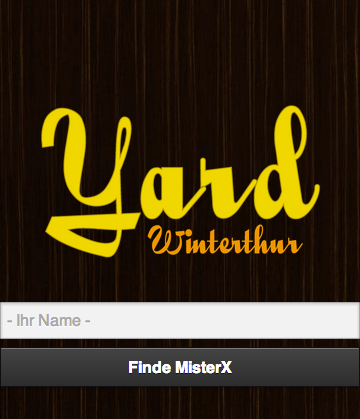
\includegraphics[width=5cm]{Bilder/login.png}

\subsection{Kartenanzeige}
Hat der Spieler sich erfolgreich eingeloggt, sieht er einen  Kartenausschnitt der Winterthurer Altstatt. Seine eigene Position ist 
mit einem roten Icon markiert.  \\ 

Auf der Karte liegt ein Graph mit verschiedenen Knoten. MisterX bewegt sich jede Minute einen Schritt von einem Knoten zum nächsten.  \\

Die Karte wird live bezogen von Open Street Map\footnote{http://www.openstreetmap.org}. Für die Darstellung wurde das Framework LeafletJs \footnote{http://leafletjs.com} eingesetzt. \\
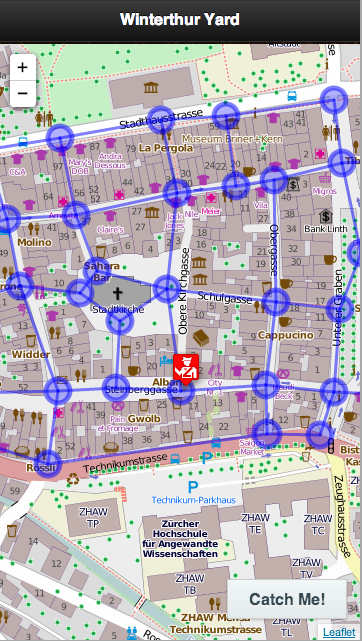
\includegraphics[width=5cm]{Bilder/rotesSymbol.png} \\
Da die Strassen nicht gerade sind, haben wir in der Datenbank die Möglichkeit einer Strecke Zwischenpunkte hinzuzufügen.  \\
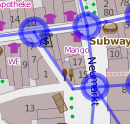
\includegraphics[width=5cm]{Bilder/strassenecke.png}

\subsection{Catch Me}
Befindet sich der Spieler auf einem der eingezeichneten Koordinaten-Punkte, kann er den Button ``Catch Me`` drücken. 

Solange sich der Spieler nicht auf einem gültigen Spielfeld (innerhalb eines Kreises auf der Karte) befindet, erhält er eine entsprechende Meldung. 

Ist der Spieler auf einem gültigen Spielfeld, wird ihm die Position von MisterX vor seinem letzten Spielzug angezeigt (roter Kreis). 

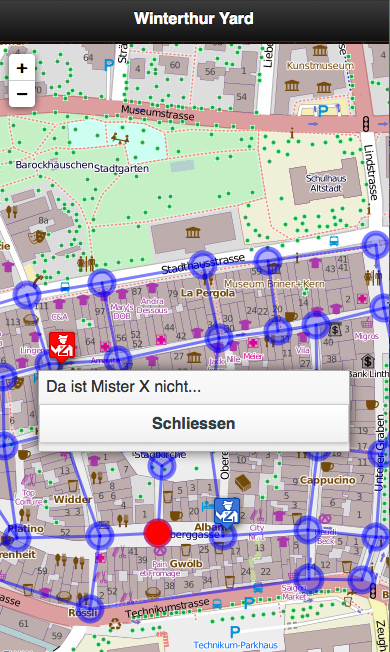
\includegraphics[width=5cm]{Bilder/MeldungMisterXNicht.png}

Zudem sieht man mit blauen Symbolen, wo sich andere Spieler aufhalten. 

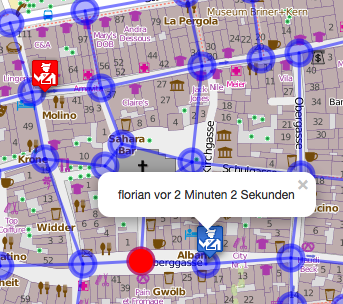
\includegraphics[width=5cm]{Bilder/AndererSpieler.png}


Drückt man zweimal auf ``Catch Me`` auf dem selben Feld, wird man darauf hingewiesen, dass dies nicht erlaubt ist. 

Wenn der Spieler sich auf dem selben Feld befindet wie MisterX erhält er eine Information, dass er MisterX gefangen hat. Das Spiel ist damit beendet. 


\section{Aufbau der Applikation}

\subsection{JavaScript}
Das JavaScript wurde alles unter yard gekapselt. Im Nachhinein gesehen, wäre es sinnvoll gewesen mehrere Objekte (z.B. Benutzer, Karte) zu erstellen. 

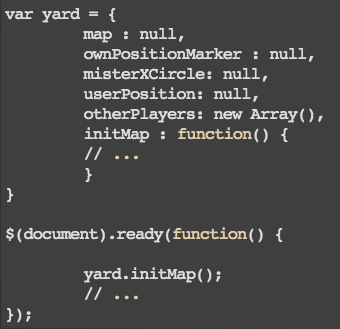
\includegraphics[width=5cm]{Bilder/AufbauJS.png}

\subsection{Kommunikation zum Server}
Die Kommunikation zum Server funktionierte über eine REST-Schnittstelle mit JSON. So konnten sehr einfach Daten übertragen werden. 

Die ganze Logik, die bestimmt, ob eine Person an einem Knoten ist, geschieht auf dem Server. Bei einem Catch Me schickt JavaScript lediglich die aktuelle Position an den Server. Dieser gibt danach eine entsprechende Antwort.

\subsection{Datenbank}
Die Datenbank wurde nach folgenden Modell aufgebaut:

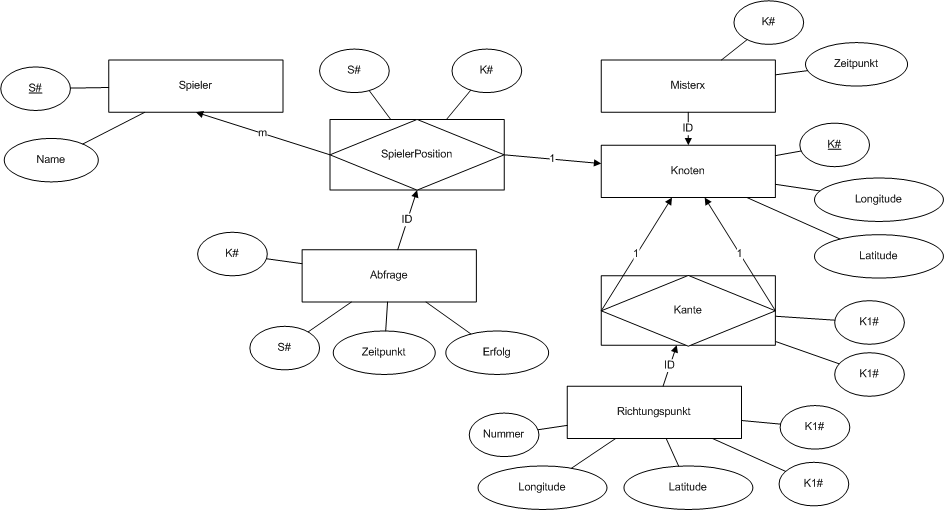
\includegraphics[width=15cm]{Bilder/ERYard.png}

\section{Erweiterungen}
Die Projektziele konnten erfüllt werden - das Spiel ist lauffähig. 

Offene Punkte und Erweiterungen
\begin{itemize}
\item Schlussendlich soll MisterX die Koordinaten eines Geocaches kennen. Zuerst muss aber ein geeignetes Versteck für den Cache in Altstadtnähe gefunden werden.

\item Über einen Button soll die Karte um den eigenen Standort zentriert werden. Im Moment ist das Zentrum immer bei der Stadtkirche Winterthur
\item Über einen Button soll die Kartenanzeige zum roten Punkt (Position von MisterX vor dem letzten Zug) springen. Dies nur, wenn dies überhaupt angezeigt wird. Ansonsten ist der Button disabled. 
\end{itemize}




\section{Fazit}
Es hat sehr viel Spass gemacht die App zu erstellen. Wir konnten diverse für uns neue Tools ausprobieren: 

\subsection{JQuery Mobile}
JQuery Mobile hat uns nicht vollständig überzeugt. Wir hatten grosse Schwierigkeiten mit dem Styling und mit der Positionierung der Karte. Deshalb haben wir das Layout, dass wir am Anfang bestimmt haben auch nicht vollständig umgesetzt. Schön ist, dass man Controls out of the box einsetzen konnte - so zum Beispiel die Popup-Mitteilungen. 

\subsection{LeafletJS}
LeafletJS hat uns sehr überzeugt dank einer einfachen und gut dokumentierten API. So hatten wir keinerlei Probleme die Karte mobile-tauglich darzustellen. 

\subsection{Slim}
Slim hat uns sehr unterstützt sauberer Webservices anzubieten. Bei unserem Billig-Hoster haben wir etwas mit mod rewrite gekämpft, dass bei Slim standardmässig verwendet wird. 

\subsection{RevealJS}
RevealJS hat uns sehr gefallen. Es ist mit sehr einfachen Mitteln möglich eine ansprechende Präsentation zu machen. Da diese auf HTML basiert, können alle Vorteile der Sourcekontrolle auch dort verwendet werden (History, Kollaboratives Arbeiten). Aus dem selben Grund haben wir unsere Dokumentation auch mit \LaTeX erstellt. 


\end{document}
